\subsubsection{Какова совокупность параметров вторичного источника питания? Дать им определение}

Питание электрической энергией устройств измерительной техники, электроники, ЭВМ и автоматики очень редко удается осуществить непосредственно от первичного источника электроэнергии. Это обусловлено тем, что стандартная электрическая сеть или автономный первичный источник электрической энергии обычно непригодны для питания электронных устройств из-за их несоответствия требованиям по величине напряжения, его стабильности, форме, частоте. Поэтому в большинстве случаев приходится применять источники вторичного питания. Под этим термином обычно понимаются преобразователи вида электрической энергии, которые выполняют нужные преобразования.

ИВЭП принято характеризовать следующим рядом показателей и признаков:
\begin{itemize}
\item Условия эксплуатации
\item Параметры входной и выходной электрической энергии
\item Выходная мощность
\item КПД
\item Время непрерывной работы
\item Время готовности к работе
\item Число каналов и пр.
\end{itemize}

Электрические показатели ИВЭП принято делить на две группы: \textbf{Статические}, определяемые при медленном изменении во времени возмущающих факторов и \textbf{Динамические}, определяемые при ...

Cтатические электрические показатели ИВЭП в общем случае имеют следующие характеристики:
\begin{itemize}
\item Номинальное значение питающего напряжения(чаще всего 220-380В) и номинальные значения выходных напряжений. 
\item Допускаемые отклонения напряжения первичной питающей сети от номинального значения
\item Номинальная частота питающего напряжения
\item Номинальные токи нагрузки
\item Суммарная мощность, отдаваемая в нагрузку
\item Нестабильность выходного напряжения при изменении напряжения питания: (Определяется как отношение изменения выходного напряжения к номинальному его значению)
$$
\delta_{U_{out(U)}} = \frac{\pm\Delta U_{out(U)}}{U_{out}}100\%
$$
\item Нестабильность выходного напряжения при изменениях тока нагрузки. (аналогично см. выше)
\item Нестабильность выходного напряжения во времени. (аналогично см. выше)
\item Температурный коэффициент выходного напряжения:
$$
TKH =  \frac{\pm\Delta U_{out(T)}}{U_{out}\Delta T}100\%
$$
\item Один из самых важных показателей - Коэффициент стабилизации по напряжению. Показывает, во сколько раз относительное приращение выходного напряжения меньше относительного приращения данного возм. фактора:
$$
K_s = \left( \frac{\Delta U_{in}}{U_{in}}\right) / \left( \frac{\Delta U_{out}}{U_{out}}\right)
$$
\item Способность стабилизированного источника уменьшать переменную составляющую на выходе $U_{out_P}$ по отношению к ее значению на входе $U_{in_P}$. Характеризуется коэффициентом сглаживания пульсаций $K_p$. Коэффициент пульсации - отношение амплитуды первой гармоники разложения сигнала в спектр к среднему значению сигнала. Фактически, $K_p$ есть отношение этих дел на входе к выходу.
$$
K_p = \left(\frac{U_{in_P}}{U_{in}}\right) / \left( \frac{U_{out_P}}{U_{out}}\right)
$$
\end{itemize}

Так выглядит схема простейшего ИВЭП:
\begin{center}
	\begin{figure}[h!]
		\center{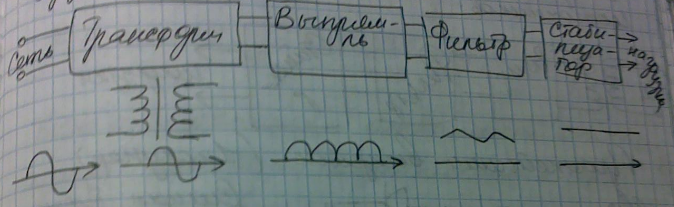
\includegraphics[scale=0.7]{Ist.png}}
		\caption{}
	\end{figure}
\end{center}
\pagebreak

